\documentclass{article}
\usepackage[pdfusetitle,pdflang=en-UK]{hyperref}
\usepackage{graphicx} % Required for inserting images
%\usepackage[sort&compress,numbers]{natbib}
%\usepackage{pdfcomment}
%\usepackage{amsmath}
\usepackage{fancyvrb}
\renewcommand{\familydefault}{\sfdefault}
\usepackage[a4paper, total={6in, 8in}]{geometry}
\usepackage[UKenglish]{datetime}
\usepackage[tagged, highstructure]{accessibility}


\title{Machine-Learned Potentials \\ Workshop 8, Data Science in Chemistry}
\author{Alan M. Lewis}

\date{}

\begin{document}

\maketitle

\section{Getting Started}

To get started, you should log into Viking using \verb|ssh -X your-username@viking.york.ac.uk|, using your usual University username and password. You should then clone the repository containing the data for this workshop by running
\begin{Verbatim}
    git clone https://github.com/alanmlewis/ml-workshop
\end{Verbatim}
This will create a new folder called ml-workshop; change directory into that folder. Everything else we do in the workshop will take place in this folder or a subfolder. Before you go any further, you should run the commands
\begin{Verbatim}
    export OMP_NUM_THREADS=1
    export OPENBLAS_NUM_THREADS=1
\end{Verbatim}
to ensure you only use 1 CPU for each calculation on the head node. You should then create a virtual environment to install all the software we will need into:
\begin{Verbatim}
    module load Python/3.10.8-GCCcore-12.2.0
    python3 -m venv ./venv
    source venv/bin/activate
\end{Verbatim}
You will then need to install \verb|gap_fit|, the software which we will use to predict energies and forces, by running
\begin{Verbatim}
    python3 -m pip install numpy==1.26.3 ase==3.22.1 quippy-ase
\end{Verbatim}
This should install \verb|gap_fit| and all of its dependencies. You may see a warning when you install, which says something to the effect that certain programs are not on PATH. In this case, please run:
\begin{Verbatim}
    export PATH=$PATH:~/.local/bin
\end{Verbatim}
To test this has installed correctly, run
\begin{Verbatim}
    gap_fit config_file=gap_config.cfg 2> /dev/null
\end{Verbatim}
This program should take a few seconds to complete, during which time you should see a lot of text produced, with the words 'Bye Bye' displayed near the end of this text.

\section{Learning Energies and Forces}

The program \verb|gap_fit| takes some input data stored in an xyz file, and trains a machine-learned potential which can be used to calculate the energy and forces of a similar target system given only the atomic positions of that target system. That input data consists of a series of snapshots of atomic positions, the associated energy of that snapshot, and the electronic forces which act on each atom. The potential produced is stored in a single file, called \verb|gap.xml|. It is very straightforward to run the program from the command line:
\begin{Verbatim}
    gap_fit config_file=gap_config.cfg 2> /dev/null
\end{Verbatim}
This reads a configuration file, here called \verb|gap_config.cfg|, which specifies where the program should look for its training data and several other parameters which govern the machine learning model. These parameters include the SOAP parameters, kernel types, and an overfitting parameter:
\begin{itemize}

\item \verb|atoms_filename|, which specifies the file which contains the training data.
\item \verb|cutoff| and \verb|atom_sigma|, which determine the radius of the atomic environment and the width of the Gaussian used to represent the atoms in that environment, respectively.
\item \verb|l_max| and \verb|n_max|, which govern the precision with which the atomic environments are quantified (larger integers = more precise).
\item \verb|covariance_type|, how the kernels are calculated. Options are \verb|DOT_PRODUCT| (linear kernel), \verb|ARD_SE| (Gaussian kernel), \verb|PP| (piecewise polynomial kernel).
\item EITHER \verb|zeta|, which determines the power to which a non-linear in the kernel is raised (if \verb|covariance_type| is \verb|DOT_PRODUCT|, default = 2), OR \verb|theta_uniform|, the width of Gaussian function used in exponential kernels (if \verb|covariance_type| is \verb|ARD_SE| or \verb|PP|, default = 1.0).
\item \verb|default_sigma| specifies how precisely we should fit to the training energies and forces (smaller values = more precise).
\item \verb|gp_file| gives the filename where the trained potential will be stored.

\end{itemize}

The following keywords must also be present in the config file, but refer to more technical details which we will not cover today and do not need to be changed.

\begin{itemize}
\item \verb|n_sparse|, the number of atomic environments to use in the training. We will always use fewer than 8000.
\item \verb|delta|, scaling parameter of the kernel per descriptor.
\item \verb|e0| contains the energies of isolated H and O atoms.
\item \verb|sparse_jitter| controls the numerical convergence of the training.
\item \verb|sparse_separate_file=F| prevents unnecessary extra files being written. 
\end{itemize}

We have covered most of these parameters in principle during the last lectures, and will now look at the effect of how varying some of these parameters affects our ML performance.

\subsection{How accurate is my model?}

In the \verb|ml-workshop| folder, you will see two python scripts, called \verb|gap_error_validate.py| and \verb|gap_error_train.py|. These perform validation on two different sets of snapshots - a validation set contained in \verb|gap_validate.xyz|, and the set of snapshots we used to train the model, respectively. These python scripts will return the root mean square error in the energy across the set of the snapshots. They also produce two files called \verb|validation_errors.csv| and \verb|train_errors.csv|, which contain the true values of the energy for each snapshot in the first column and the corresponding predicted energy in the second column. To run these scripts, just type \verb|python3 script_name.py|.

\subsubsection*{Exercises}

\begin{enumerate}
 
\item Train a GAP model using the default parameters in the \verb|gap_config.cfg| file.
\item What is the RMSE in the predicted energies of the validation set?
\item What is the RMSE in the predicted energies of the training set?
\item Why are these values different?
\end{enumerate}

\subsection{Creating a Learning Curve}

The most important way to test whether our machine learning method is working as we expect is to plot a learning curve - that is, a plot of the RMSE in the predictions of the model against the number of snapshots used to train the model. We expect to see the error decrease as the number of training snapshots is increased, up to some limit when the error stops reducing.

To help you plot a learning curve using \verb|gap_fit|, a number of input files are provided labeled \verb|gap_input_N.xyz|, where \verb|N| is the number of snapshots in the training set. Each set includes all of the snapshots in the previous set, plus some new snapshots. You can select your training set by modifying \verb|gap_config.cfg|.

In general, \textbf{we shouldn't run calculations on the head node of Viking}. Included in the directory is a submission script called \verb|sub.sbatch|, which will run \verb|gap_fit|, followed by the two python scripts which calculate the error on the validation set and the training set. The output from \verb|gap_fit| is stored in a file called \verb|GAP.out|, while the errors on the validation set are stored in \verb|errors.out|.

\subsubsection*{Exercises}

\begin{enumerate}

\item Train a model using 50, 100, 200 and 400 snapshots. After training each one, calculate the accuracy of each model on both the validation set and the corresponding training set, making a note of each error as you go.
\item Plot the learning curves for both the RMSE over the training set and validation set on a single graph. Does what you see match your prediction from the previous section?

\end{enumerate}

\subsection{Overfitting}

Overfitting is a common problem when performing machine learning. It describes a situation where a model can extremely accurately reproduce the data in your training set, but in doing so is extremely unpredictable and inaccurate "between" the training points. This is illustrated in Figure 1.

\begin{figure}[t]

\centering

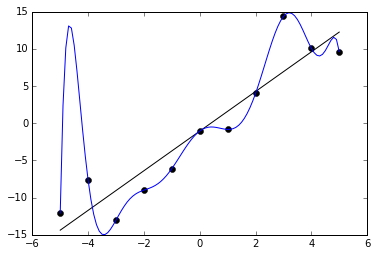
\includegraphics[width=0.7\textwidth]{Overfitted_Data.png}
\caption{A graph illustrating the concept of overfitting. The blue line goes through all of the known points (training data) very closely, but using this function to interpolate values between the known results is likely to produce very poor predictions. By contrast, the black line does not reproduce the training data precisely, but gives more accurate interpolation. Image Credit: \href{https://en.wikipedia.org/wiki/Overfitting}{Wikipedia}.}

\end{figure}

Overfitting can be caused by a poor choice of a number of parameters. Some of these are directly connected to the idea of overfitting. For example, in \verb|gap_config.cfg|, the first value in the variable \verb|default_sigma| is an estimate of the standard deviation in the energy calculations. This effectively tells the model how closely it should try to fit to the training data. A small value here will almost always lead to overfitting. However, sometimes other parameters can lead to overfitting in less obvious ways. For example, having extremely accurate descriptions of the atomic environments (determined by \verb|nmax| and \verb|lmax| in \verb|gap_config.cfg|) can lead to overfitting.

Note that if you want to save the GAP models you train with certain parameters, you will need to change the \verb|gp_file| keyword before you run \verb|gap_fit|, otherwise the model will be saved to \verb|gap.xml| every time, overwriting the previous model. However, if you do this you will also need to modify the python files you run to ensure that you load the correct model (all python files will load \verb|gap.xml| by default).

\subsubsection*{Exercises}

\begin{enumerate}
\item How could you identify when overfitting is taking place?
\item Using 100 training snapshots, train models using different values of \verb|default_sigma| for the energy and calculate the RMSE on the training and validation set each time. Do the results match your expectations? What is the optimal value, in your opinion?
\item Repeat this exercise varying the cutoff radius of the SOAP descriptors, the number of radial functions used to describe the SOAP environment, and the type of kernel used in the calculation. Do these affect the accuracy of the model? Can they cause overfitting? What is the optimal value, in your opinion?
\item Once you have found the optimal value of some parameter(s), use these parameters to train a model using 200 snapshots. Does this lead to more or less overfitting than when you used 100 snapshots? Is the difference significant?

\end{enumerate}

\subsection{Running Molecular Dynamics with an ML Potential}
\label{sec:md}

So far we have only considered the energy predicted by the ML model, but the model also predicts the forces exerted on each atom by the electrons in the molecule. This means that once we have trained a machine learning model which we are happy is sufficiently accurate, we can use it to run molecular dynamics simulations. The simple script \verb|molecular_dynamics.py| does exactly that: it takes a snapshot from the validation set as a starting point, randomly assigns velocities to each atom, and uses the machine learned potential to calculate the forces acting on each atom. That is all of the information required to perform a dynamics simulation, as we use these velocities and forces to calculate the atomic positions and velocities a short time later, and then recalculate the forces on the atoms in their new positions using the ML potential. Doing this repeatedly results in a molecular dynamics trajectory.

\subsubsection*{Exercises}

\begin{enumerate}

\item Read through through the python script \verb|molecular_dynamics.py| and make sure you understand what each command does.
\item Using the submission script \verb|md_sub.sbatch|, run a molecular dynamics simulation for 200 timesteps at constant energy, and check the logfile \verb|nve.log| which is produced. What information in this log file could you use to establish if your ML potential is working as expected or not?
\item Run a molecular dynamics simulation with a thermostat for 100 timesteps, and check the logfile \verb|nvt.log| which is produced. You will see that the total energy of the system is not conserved. What real-life experimental conditions are we reproducing which explains this variation in the total energy?
\item The dynamics calculated using the ML potential are approximately 1400 times faster than the traditional MD simulation I performed to obtain the training data. However, that doesn't account for the time it takes to create the model in the first place. What additional timings do we need to know to make a truly fair comparison of the computation costs of the two approaches? When will it be worth training an ML model to perform dynamics?

\end{enumerate}


\subsubsection*{Visualising the Trajectory}

The trajectory produced by running a MD simulation is saved in the file \verb|trajectory.xyz|. This can be visualised using software called VMD. Load this software by running \verb|module load VMD|, then load the trajectory using the command \verb|vmd trajectory.xyz|. This will open two windows - a visualisation, and a control window. For the best visualisation, from the control window choose Graphics, then Representations, which will open a new window. In this window find the dropdown menu for Drawing Method, and select VDW. Close this window, and use the play button in the bottom right of the control window to visualise the trajectory.

\end{document}
